\chapter{Implementierung}

Die Implementierung ist in drei Teile gegliedert. Zunächst wird die Extraktion und Speicherung der Features näher beschrieben. Im Anschluss wird der Aufbau der Modelle behandelt. Im zweiten Teil wird die Umsetzung des Bag of Visual Word Modells in CUDA C betrachtet. Im Wesentlichen werden hier die \textit{kernels} für den k-means Algorithmus angeführt sowie Unterschiede in der Implementierung zwischen \textit{global} und \textit{shared memory} behandelt. Der dritte Abschnitt illustriert eine Autoencoder Implementierung in TensorFlow. 

\section{Feature Extraktion}

Da es sich bei der Feature Extraktion für beide Modelle um einen Schritt zur Vorverarbeitung handelt, würde eine Umsetzung genügen. Die beiden Umgebungen der Umsetzung unterschieden sich jedoch sehr voneinander: CUDA C ist eine sehr hardwarenahe Sprachen, Python ist eine interpretierte Hochsprache und TensorFlow generiert den entsprechenden Code für die Grafikkarte automatisch aus einem Modell. Aus diesem Grund wird eine Funktion zur Extraktion in beiden Sprachen bereitgestellt. Intern wird aber bei beiden auf die \textit{opencv}\footnote{https://github.com/TODO/opencv} Implementierung von SIFT zurückgegriffen. Zur Verwendung des SIFT Algorithmus ist es erforderlich das \textit{opencv} Projekt zusammen mit dem \textit{opencv-contrib}\footnote{https://github.com/TODO/opencv-contrib} Projekt selbst zu kompilieren. Bei SIFT handelt es sich um einen patentierten Algorithmus, daher ist er seit Version 3.0 nicht mehr standardmäßig im \textit{opencv} Projekt enthalten. 

In C wird zur Gewinnung der Feature-Vektoren eines Bildes \textit{extractFeatures} mit dem Pfad des Bildes aufgerufen. Die vollständige Funktion kann nachfolgendem Codelisting entnommen werden. Um die Übersicht zu wahren, wurde hier auf die Importe verzichtet. Neben den \textit{opencv} Standardimporten ist es jedoch zusätzlich notwendig \textit{opencv/nonfree/features2d} einzubinden. Zunächst wird das Bild durch \textit{opencvs} \textit{imread} Methode eingelesen und liegt im Speicher als Matrix vor. Da SIFT mit monochromatischen Bildern arbeitet, wird vor der Detektion das eingelesen Bild konvertiert. Um hieraus die Deskriptoren zu berechnen, bietet \textit{opencv} eine \textit{SiftFeatureDetector} Klasse an. Via \textit{detect} werden im ersten Schritt die \textit{keypoints} ermittelt (Zeile 8) und in Zeile 9 aus dem Bild und den \textit{keypoints} die Deskriptoren berechnet. Die Deskriptoren werden dann als \textit{opencv} Matrix zurückgegeben.

\lstset{language=C}
\begin{lstlisting}
using namespace cv;

Mat extractFeatures (String imagePath) {
	const Mat image;
	const Mat source = imread(imagePath, 0);
	cvtColor(source, image, CV_RGB2GRAY);
	SiftFeatureDetector detector;
	vector<KeyPoint> keypoints;
	Mat descriptors;
	
	detector.detect(input, keypoints);
	detector.compute(input, keypoints, descriptors);
	return descriptors;
}
\end{lstlisting}

\section{Ansatz 1: Bag of Visual Words}

Das Bag of Visual Words Modell wurde direkt in CUDA C umgesetzt. Sofern die Deskriptoren aus den Trainingsbildern extrahiert wurden, kann durch \textit{generateModel} die Generierung eines Modells gestartet werden. Hier werden die Features, die Anzahl der Cluster und eine Referenz auf eine Liste von Mitgliedschaften erwartet. Neben den Schwerpunkten der Cluster werden die Mitgliedschaften berechnet: Pro Cluster liegt eine Liste vor, die alle \textit{keypoints}, die zu dem Cluster gehören, enthält. Sowohl die Schwerpunkte der Cluster als auch die Mitgliedschaften werden nach der Verarbeitung auf die Festplatte in verschiedene Dateien geschrieben. Die Schwerpunkte der Cluster werden zeilenweise in die Datei \textit{modelPath}/clusters geschrieben, sodass sich $k$ Zeilen mit 128 Elementen bei der Verwendung von SIFT ergeben. Die Mitgliedschaften der Features zu Cluster wird in der Datei \textit{modelPath}/membership gespeichert und enthält so viele Zeilen wie Features vorliegen. Jede Zeile enthält die $x$ und $y$ Koordinaten des \textit{keypoints} und den Index des zugehörigen Clusters. Der Index bezieht sich hierbei auf die Position des Clusters in der Datei \textit{modelPath}/clusters.

\subsection{Paralleler k-means Algorithmus}

Als Referenzimplementierung für die Umsetzung in CUDA C diente hier das Projekt von \todo{[REF]}. Der Algorithmus erwartet einen Feature-Vektor, die Feature-Dimension und die Anzahl der zu bildenden Cluster als Eingabe. Vor dem Aufruf des \textit{kernels} wird für die Features und Cluster der notwendige Speicher allokiert und die Daten zum \textit{device} kopiert. Die Dimensionen der Features sowie der Cluster werden durch \textit{Float}-Werte dargestellt, sodass ein SIFT Feature-Vektor bzw. der Schwerpunkt eines Clusters $128 \times 4$ Byte $= 512$ Byte belegt. Da die Features ursprünglich als zweidimensionales Array vorliegen (\textit{Float-Pointer-Pointer}), müssen diese in ein eindimensionales Arrays konvertiert werden, damit die Daten korrekt von \textit{host} zu \textit{device} kopiert werden können. 

\subsubsection{Global memory}

Die in der Konzeption vorgestellten Funktionen sind als Funktion in C umgesetzt worden. Von diesen sind drei CUDA kernels, also Funktionen die durch die Grafikkarte ausgeführt werden. Diese Funktionen werden solange in einer Schleife durchlaufen, bis das Konvergenzkriterium erfüllt wurde.

\begin{itemize}
	\item \textbf{Distanzberechnung} euclideanDistance(float *points, float *clusters)
	\item \textbf{Cluster-Mitgliedschaft} findNearestCluster() agiert auf jeweils einem Feature. Der Index des Features ist somit von der $threadIdx$ abhängig und berechnet sich unter Berücksichtigung der Blockdimension als $blockDim.x * blockIdx.x + threaIdx.x$. Es wird der nächste Cluster zum Feature bestimmt und auch berechnet, ob sich die Zuordnung des Features verändert hat. \todo{Parallel reduction}
	\item \textbf{Konvergenzkriterium} computeDelta() ermittelt die Anzahl der Veränderungen der Feature-Cluster Mitgliedschaft. Im wesentlichen werden durch eine  parallele Reduktion die Veränderungen die in \textit{intermediates} festgehalten wurden aufsummiert.
\end{itemize}

Die Anzahl der veränderten Mitgliedschaften wird anschließend zurück zum \textit{host} kopiert. Diese Zahl wird durch die Gesamtanzahl der Features dividiert, um so die relative Veränderung zu bestimmen. Ist diese kleiner als ein vorgegebener Schwellwert oder wurde eine maximale Anzahl an Iterationen erreicht, ist das Clustering abgeschlossen, andernfalls wird fortgefahren.

\subsubsection{Shared memory}

Zur Beschleunigung der Berechnung bei der Suche des nächsten Clusters zu einem gegebenen Punkt, soll CUDAs \textit{shared memory} genutzt werden. Hierfür werden die Cluster pro Block vom \textit{global} in den \textit{shared memory} kopiert. Daraus ergibt sich eine Anpassung an mehreren Stellen im Programm. Die Größe des extra zu allokierenden Speichers pro Block muss in \textit{blockSharedDataSize} berücksichtigt werden und ergibt sich aus der Anzahl der Cluster und der Anzahl der Elemente eines Features:

\lstset{language=C}
\begin{lstlisting}
const unsigned int membershipDataSize = numThreads * sizeof(unsigned char);
const unsigned int clusterDataSize = k * size * sizeof(float);
const unsigned int blockSharedDataSize = membershipDataSize + clusterDataSize;
\end{lstlisting}

In der Funktion \textit{findNearestCluster} wird der Parameter \textit{clusters} in \textit{deviceClusters} umbenannt. Vor der Berechnung der Mitgliedschaft wird nun ein lokaler Pointer \textit{clusters} angelegt und alle notwendigen Cluster kopiert.

\lstset{language=C}
\begin{lstlisting}
float *clusters = (float *)(sharedMemory + blockDim.x);
for (int i = threadIdx.x; i < k; i += blockDim.x) {
  for (int j = 0; j < size; j++) {
    clusters[k * j + i] = deviceClusters[k * j + i];
  }
}
__syncthreads();
\end{lstlisting}

Da die Größe von \textit{clusterDataSize} hier von $k$ und $size$ abhängt, also der Anzahl der Cluster und der Anzahl der Komponenten eines Features, ist diese Implementierung nur einsetzbar, wenn $k$ und $size$ in Hinsicht auf den verfügbaren \textit{shared memory} nicht zu groß gewählt werden. Die Größe von \textit{membershipDataSize} ist nur abhängig von der Anzahl der Threads. Werden beispielsweise 256 Threads pro Block gewählt, benötigt dies konstant, unabhängig von $k$ und $size$, 1024 Byte \textit{shared memory}. Durch die Verwendung von SIFT ist die Anzahl der Komponenten von Features auf 128 festgelegt, sodass letztendlich eine Obergrenze für $k$ berechnet werden kann. Gängige Modelle CUDA kompatibler Grafikkarten sind mit 16 oder 48 Kilobyte \textit{shared memory} ausgestattet. Von 256 Thread pro Block ausgehend ergibt dies ein maximales $k$ von $(memory - 1024) / 512$. Dies sind bei 48 Kilobyte maximal 91, für 16 Kilobyte 29 Cluster. Für viele praktische Anwendungsfälle ist dies bereits ausreichend. Sind dennoch mehr Cluster notwendig, muss auf die \textit{global memory} Implementierung zurückgegriffen werden. Hier werden, je nach Anzahl der Cluster, erheblich höhere Berechnungszeiten erwartet, jedoch gibt es kein Limit für die Gesamtanzahl an Clustern.

\section{Ansatz 2: Autoencoder}

In diesem Kapitel wird behandelt wie der Autoencoder in Python und TensorFlow umgesetzt wurde. Zunächst wird auf die Erhebung der Feature-Vektoren unter Verwendung der \textit{opencv}-Bibliothek eingegangen. Anschließend erfolgt eine Übersicht des Python-Codes zur Definition des Autoencoders.

\subsection{Erhebung der Feature-Vektoren}

Um die 3042-elementigen Feature-Vektoren zu extrahieren, wurde hier ebenfalls die \textit{opencv}-Bibliothek genutzt. Der Prozess lässt sich in drei Schritte untergliedern. Um alle Features eines Bildes zu erhalten, wird die Funktion \textit{extractFeatures} mit dem Pfad zu einer Bilddatei ausgerufen. Es wird das Bild eingelesen, konvertiert und durch den \textit{opencv} SIFT-Detektor die \textit{keypoints} ermittelt. Die Berechnung der Gradienten der Nachbarschaften um diese \textit{keypoints} erfolgt dann durch die Funktion \textit{computeDescriptors}:

\lstset{language=Python}
\begin{lstlisting}
def computeDescriptors(image, keypoints):
  descriptors = []
  
  for keypoint in keypoints:
  	patch = getPatch(image, keypoint)
  	gradients = computeGradients(patch)
  	descriptors.append(gradients)
  return descriptors
  
def getPatch (image, keypoint):
  x, y = keypoint.pt[0], keypoint.pt[1]
  return image[y-20:y+21, x-20:x+21]
\end{lstlisting}

Für jeden \textit{keypoint} werden nun wiederum \textit{Patches} berechnet: Hierbei handelt es sich um die Nachbarschaften der Größe $41 \times 41$. Die Gradienten in vertikale und horizontale Richtung eines solchen \textit{Patches} werden durch \textit{computeGradients} bestimmt. In Zeile 2 und 3 in Abbildung \ref{lst:compGrad} findet die Konvolution des Patches mit dem Sobel-Operator statt, den \textit{opencv} anbietet.

\lstset{language=Python,label={lst:compGrad}}
\begin{lstlisting}
def computeGradients(image):
  grad_x = cv2.Sobel(image, cv2.CV16S, 1, 0)
  grad_y = cv2.Sobel(image, cv2.CV16S, 0, 1)
  return [grad_x, grad_y]
\end{lstlisting}

In Abbildung \ref{img:gradients} sind auf der rechten Seite sind, in zwei Reihen, einige der gefundenen Gradienten des Bildes auf der linken Seite dargestellt. Dadurch, dass das Bild des Stop-Schildes viele deutliche Kanten aufweist, sind die Gradienten leicht zuzuordnen.

\begin{figure}
	\centering
	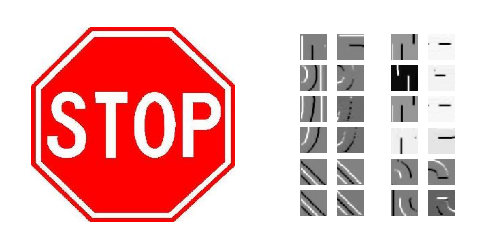
\includegraphics[scale=0.65]{images/gradients_patch.png}
	\caption{Stop-Schild und Gradienten um einige der gefundenen \textit{keypoints}.}
	\label{img:gradients}
\end{figure}

\subsection{Autoencoder Modell in TensorFlow}

Zur Implementierung des Autoencoders wurde TensorFlow verwendet. TensorFlow ist ein DeepLearning Framework und bietet Schnittstellen in diversen Sprachen an. Neben OpenCL wird auch NVIDIAs CUDA unterstützt, sodass TensorFlow Programme automatisch von Grafikkarten profitieren können, ohne das der Entwickler diese explizit berücksichtigen muss. Für diese Umsetzung eines Autoencoders wurde Python und das Projekt \textit{libsdae-autoencoder-tensorflow}\footnote{https://github.com/rajarsheem/libsdae-autoencoder-tensorflow} von Rajar Sheem genutzt. Ein simpler Autoencoder mit einem HiddenLayer lässt sich wie folgt definieren:

\lstset{language=Python}
\begin{lstlisting}
from deepautoencoder import StackedAutoEncoder
import cv2
import numpy

features = extractAllFeatures(imagePaths)
index = numpy.random.rand(features.shape[0]) < 0.8
train = features[index]
test = features[~index]

model = StackedAutoEncoder(
  dims=[3042, 1024, 512, 128, 36],
  activations=['relu', 'relu', 'relu', 'relu', 'relu'], 
  epoch=[3000, 3000, 3000, 2000, 1000], 
  loss='rmse', 
  lr=0.007, 
  batch_size=100
)

model.fit(train)
result = model.transform(test)
\end{lstlisting}

\begin{enumerate}
	\item TODO: erklären, tatsächliches Netz
	\item Referenzlayout
	\item Einlesen der Feature Vektoren etc.
	\item Speichern / Laden eines Netzes?
	\item Training
\end{enumerate}
